


An unsupervised Auto-Encoder (AE) is used to learn an optimal representation of these parameters. This is followed by a Feed Forward (FF) network which generates the final snow-cover map as a two-class classification process. The methodology consists of two parts, first the PolSAR data is transformed into basis simulated normalized stokes vectors (Section~\ref{sec:poincare_A5x}), followed by encoding and classification by an Auto-Encoder network (Section~\ref{sec:AE_A5x}).


 
\begin{figure}[!htbp]
\centering
\includegraphics[width=\textwidth]{Figures/SnowCover2018/FlowChart}
\caption{Overall description of the Neural Network.}
\label{fig:flow}
\end{figure}

\subsection{Data Preprocessing}\label{sec:method}
%\subsection{Poincar\'e sphere parameters}
\label{sec:poincare_A5x}
In PolSAR, the Mueller matrix is a real representation of backscattering measurement unlike scattering or covariance matrices which are complex. The Mueller matrix for incoherent scattering representation can be obtained from the elements of the coherency matrix $[\mathbf{T}]$ as follows:

\begin{equation}\label{incoKen}
[\mathbf{M}] =
\left[\begin{array}{cccc}
\frac{T_{11}+T_{22}+ T_{33}}{2} & \Re(T_{12}) & \Re(T_{13}) & \Im(T_{23})\\
\Re(T_{12}) & \frac{T_{11}+T_{22}-T_{33}}{2} & \Re(T_{23}) & \Im(T_{13})\\
\Re(T_{13}) & \Re(T_{23}) & \frac{T_{11}-T_{22}+T_{33}}{2} & - \Im(T_{12})\\
\Im(T_{23}) & \Im(T_{13}) & - \Im(T_{12}) &\frac{-T_{11}+T_{22}+T_{33}}{2}
\end{array}\right]
\end{equation}

The received Stokes vector $\begin{bmatrix} g_{0r} \; g_{1r} \; g_{2r} \; g_{3r} \end{bmatrix}^{T}$~\eqref{eq:stokes} is directly obtained from the observed Mueller matrix $[\mathbf{M}]$ by altering the incident Stokes vector $\begin{bmatrix} g_{0i} \; g_{1i} \; g_{2i} \; g_{3i} \end{bmatrix}^{T}$ given in table~\ref{tab:K_models}.

\begin{gather}
 \begin{bmatrix} g_{0r} \\ g_{1r} \\ g_{2r} \\ g_{3r} \end{bmatrix}
 =
  [\mathbf{M}] \cdot
 \begin{bmatrix} g_{0i} \\ g_{1i} \\ g_{2i} \\ g_{3i} \end{bmatrix}
 \label{eq:stokes}
\end{gather}

The normalized Stokes vector is given in~\eqref{eq:norm_stokes}~\cite{Shang_QNN_2014} indicates a point on or inside the Poincar\'e sphere depending on the degree of polarization. This normalized vector is used as an input feature to the neural network, $X$. 

\begin{equation}
X = (\bar{g}_{1r}, \bar{g}_{2r}, \bar{g}_{3r}) = \left(\frac{g_{1r}}{g_{0r}}, \frac{g_{2r}}{g_{0r}}, \frac{g_{3r}}{g_{0r}} \right)
\label{eq:norm_stokes}
\end{equation}

\begin{table}[tp]
\centering
\caption{Incident Stokes vector representation (H: Linear horizontal, V: Linear vertical, R: Right circular, L: Left circular)}
\label{tab:K_models}
\begin{tabular}{lcccc}
$g_{i}$ & H & V & R & L\\ \hline
$g_{0i}$ & 1 & 1 & 1 & 1 \\ 
$g_{1i}$ & 1 & $-1$ & 0 & 0 \\ 
$g_{2i}$ & 0 & 0 & 0 & 0 \\ 
$g_{3i}$ & 0 & 0 & $-1$ & $1$ \\ 
\end{tabular}
\end{table}



\subsection{Unsupervised Representation Learning using Auto-Encoders}
\label{sec:AE_A5x}
The neural network is comprised of two parts, an unsupervised AE for feature representation learning, and a supervised Feed-Forward (FF) network for supervised classification as shown in Fig.~\ref{fig:flow}. 
%
The AE has five layers: two encoding layers, two decoding layers and one representational layer, whose weights are denoted as $Z$. During training of the AE encoder, the FF network is disconnected i.e. weight updates for it are suspended. Rectified linear unit (ReLU) is used as the activation function to overcome the issue of vanishing gradients during training in a deep network.
%
The goal of the AE is to learn a representation $X'$, given input $X$. It follows that $X$ must be as close to $X'$ as possible. This governed by the cross entropy error between them during the training phase give as,

\begin{equation}
H(X,X') = E_X[-\log X'] = H(X) + D_{KL}(X||X')
\end{equation}

where $H(X)$ us the entropy of $X$, and $D_{KL}(X||X')$ is the  Kullback-Leibler divergence of $X$ from $X'$.

Training of the AE is considered complete if the  change in cross entropy error between successive iterations is negligible, or if the maximum number of iterations are exceeded. The pixels must be presented in a different randomized order each epoch, to prevent the network from memorizing the order pixels, and instead try to learn an optimal representation to simplify classification of the data.
%
After the training phase of the AE, the representational layer is extracted by applying the Poincar\'e sphere parameters and saving the weights of $Z$, in a pixel-by-pixel fashion. These extracted weights are used as input for the FF network. The AE is set up such that the dimensionality of $Z$ is greater than that of $X$. This makes the representation sparse, which can lead to improved separability between classes~\cite{coates2011importance}. 

\section{Supervised Classification}
The FF network is a three layer fully connected supervised feed forward network. The extracted representation $Z$ is given as input along with training labels to the FF network. It is trained in a supervised manner with Sigmoid nodes used as non-linearities. The training in this case is governed by the $L2$ loss. After training, the unlabeled pixels are presented to the network, and the output response is monitored. The pixel is classified into the class corresponding to the node with the highest response. 
%
Thus, a sparse unsupervised representation is learned by an AE, followed by supervised classification of this representation by a FF network. The representation is more separable than the original feature space which improves classification performance. In this paper, we use both full and hybrid polarimetric data to evaluate their effectiveness in snow cover mapping application.

\section{Dataset and Study Area}

\begin{figure}[htp]
\centering
\begin{subfigure}[b]{0.45\columnwidth}
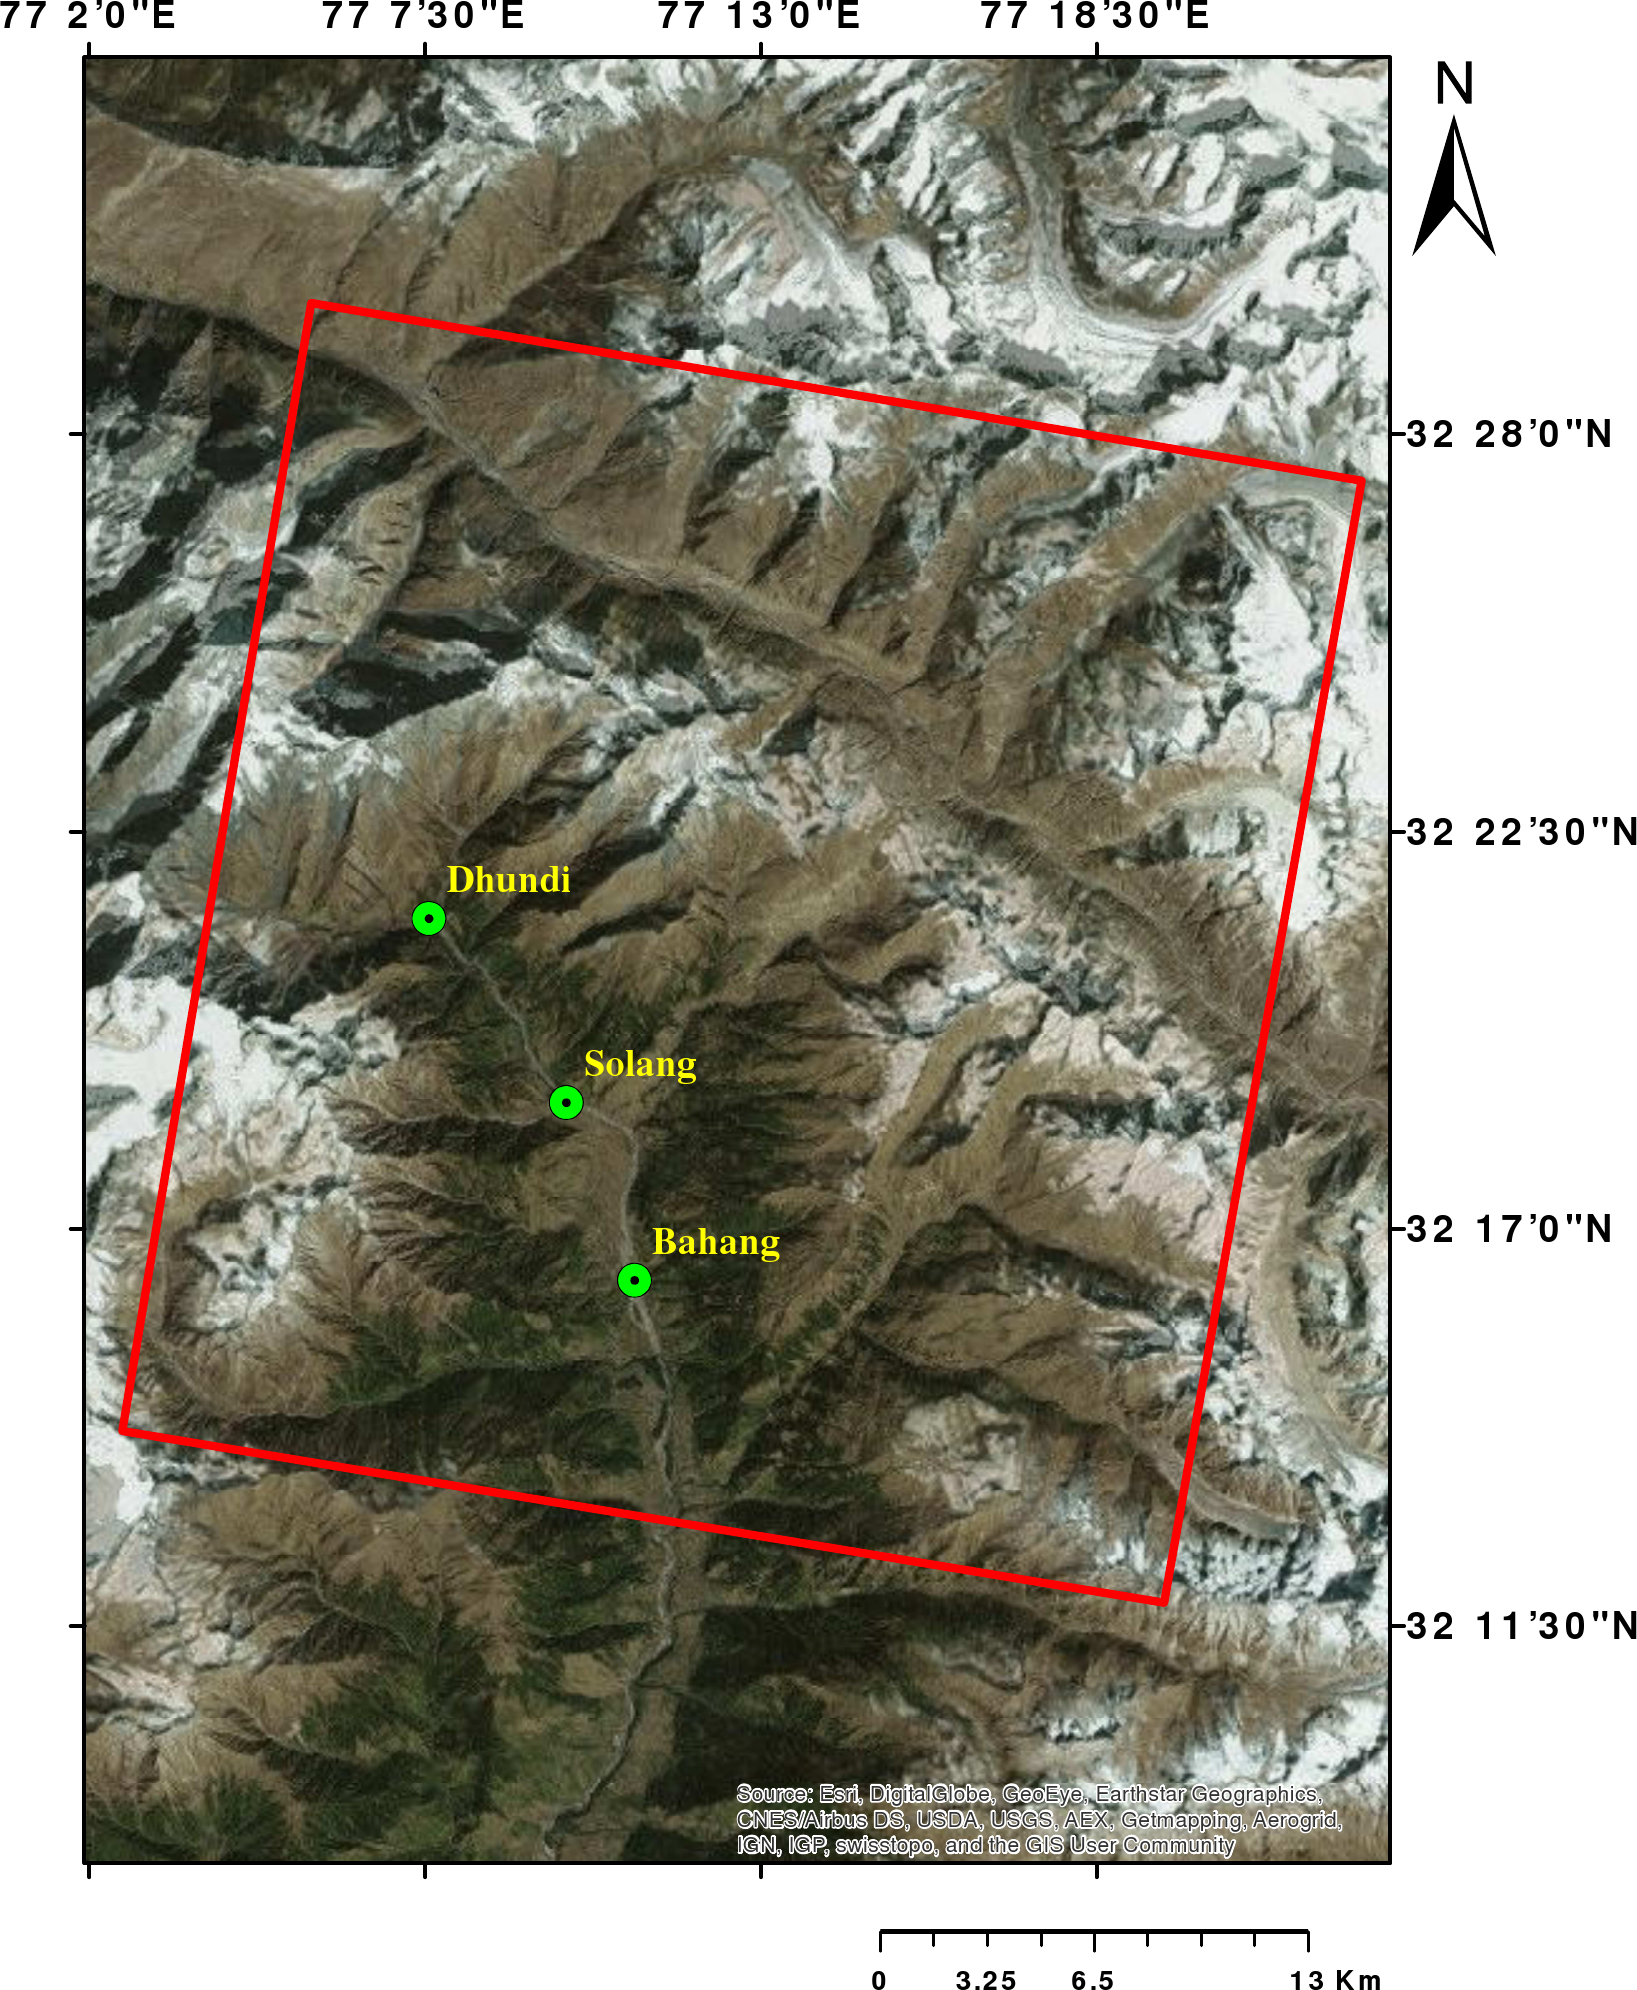
\includegraphics[width=\textwidth]{Figures/SnowCover2018/Oldfig/StudyAREA}
\end{subfigure}
\begin{subfigure}[b]{0.45\columnwidth}
\includegraphics[width=\textwidth]{Figures/SnowCover2018/Oldfig/Cropped_DEM_Manali_KML}
\end{subfigure}
\caption{(a) SAR image footprint overlaid over the study area, long with markers denoting location of the observatories. (b) Topographic variations in the region. }
\label{fig:observatory_study}
\end{figure}

%%%%%%%%%%%%%%%%%%%%%%%%%%%%%%%%%%%%%%%%%%%%%%%%%%%%%%%%%%%%%%%%%%%%%%%%%%%%%%%%%%%%Arnab Wrote
The test site is located in the Manali-Dhundi region between the latitudes of $32^{o} 11^{'} N$ to $32^{o} 30^{'} N$, and between the longitudes of $77^{o} 2^{'} E$to $77^{o} 24^{'} E$. The lower elevations of the area is covered with coniferous forest and hence there is a natural divide between areas with/without vegetation. The town of Manali is located in the bank of the river Beas which flows through the valley that contains the forest. 
%
A section of river Chenab is also captured in the scene which is housed in another valley (sparsely vegetated) located at a higher elevation. The Snow and Avalanche Study Establishment (SASE) maintains meteorological observatories over this area at differing elevations. Observatory data was used to gain a better understanding of the climate and snow conditions. The location of these observatories are marked in~Figure~\ref{fig:observatory_study} (a). Bahang observatory is at a height of $2000$  meters above sea mean level (MAMSL), Solang is $2450$ MAMSL and Dhundi is located $2900$ MAMSL.


In the Indian Himalayan region, the snowfall generally occurs during the month of December to March from an altitude of 2000 m above the mean sea level. The mean minimum temperature in the month of January is around $-15^\circ C$  to $0^\circ C$ and the mean maximum temperature in the month of June is around 2$0^\circ C$ to $30^\circ C$. The elevation fn the region varies from $1685$ MAMSL to $5020$ MAMSL, with rapid topographic variations as show in Figure~\ref{fig:observatory_study} (b). This variation in climate and altitude leads to an interesting micro-climate system to be setup in the area.  

In this study a multi-spectral scene from Landsat-8 and a SAR data-set acquired by Radarsat-2 is used. 
%
The Landsat platform carries two instruments capable of imaging in visible, infrared and near-infrared wavelengths at a spatial resolution of $30m$, pan-chromatically at $15m$ and in the thermal infrared range range at $100m$ simultaneously. The scene used in this study was acquired on the 23$^{rd}$ of March, 2015 and was the nearest concurrent cloud free acquisition available to the SAR dataset. 

The SAR scene was acquired on 18 March 2015 at 6:14 AM in the descending pass configuration with incidence angle in the range $46.0^\circ-47.2^\circ$ across the swath. The sensor was in the 'Standard Quad-Pol' yielding a $25\times25$ Km fully polarimetric measurement with HH, VV, HV and VH polarizations at a spatial resolution of 11.8m in range and 5.1m in azimuth. The coverage of the optical image is significantly greater than that of the SAR scene and has been cropped accordingly. 
%
In this time of the year the Manali-Dhundi region is mostly snow-covered except for the relatively lower altitude forested zone which remains snow-free at the canopy level.


%%%%%%%%%%%%%%%%%%%%%%%%%%%%%%%%%%%%%%%%%%%%%%%%%%%%%%%%%%%%%%%%%%%%%%%%%%%%%%%%%%%%%










